\begin{frame}
  \frametitle{Assumptions}

  \begin{itemize}
  
  \item New Nuclear = ABWRs
  
  \item Nuclear, wind, solar growth rates based on trends in USA, China, Japan.
  
  \item CCS: Available for deployment in 2030, costs reduce by 2050.
  
  \item H$_2$: Steam reforming available in 2030, photocatalytic conversion in 2050.
  
  \item Hydropower, geothermal capacity held constant.
  
  \end{itemize}

\end{frame}


\begin{frame}
  \frametitle{Cost Variation of Solar and Wind}
  \begin{figure}[htbp!]
    \begin{center}
      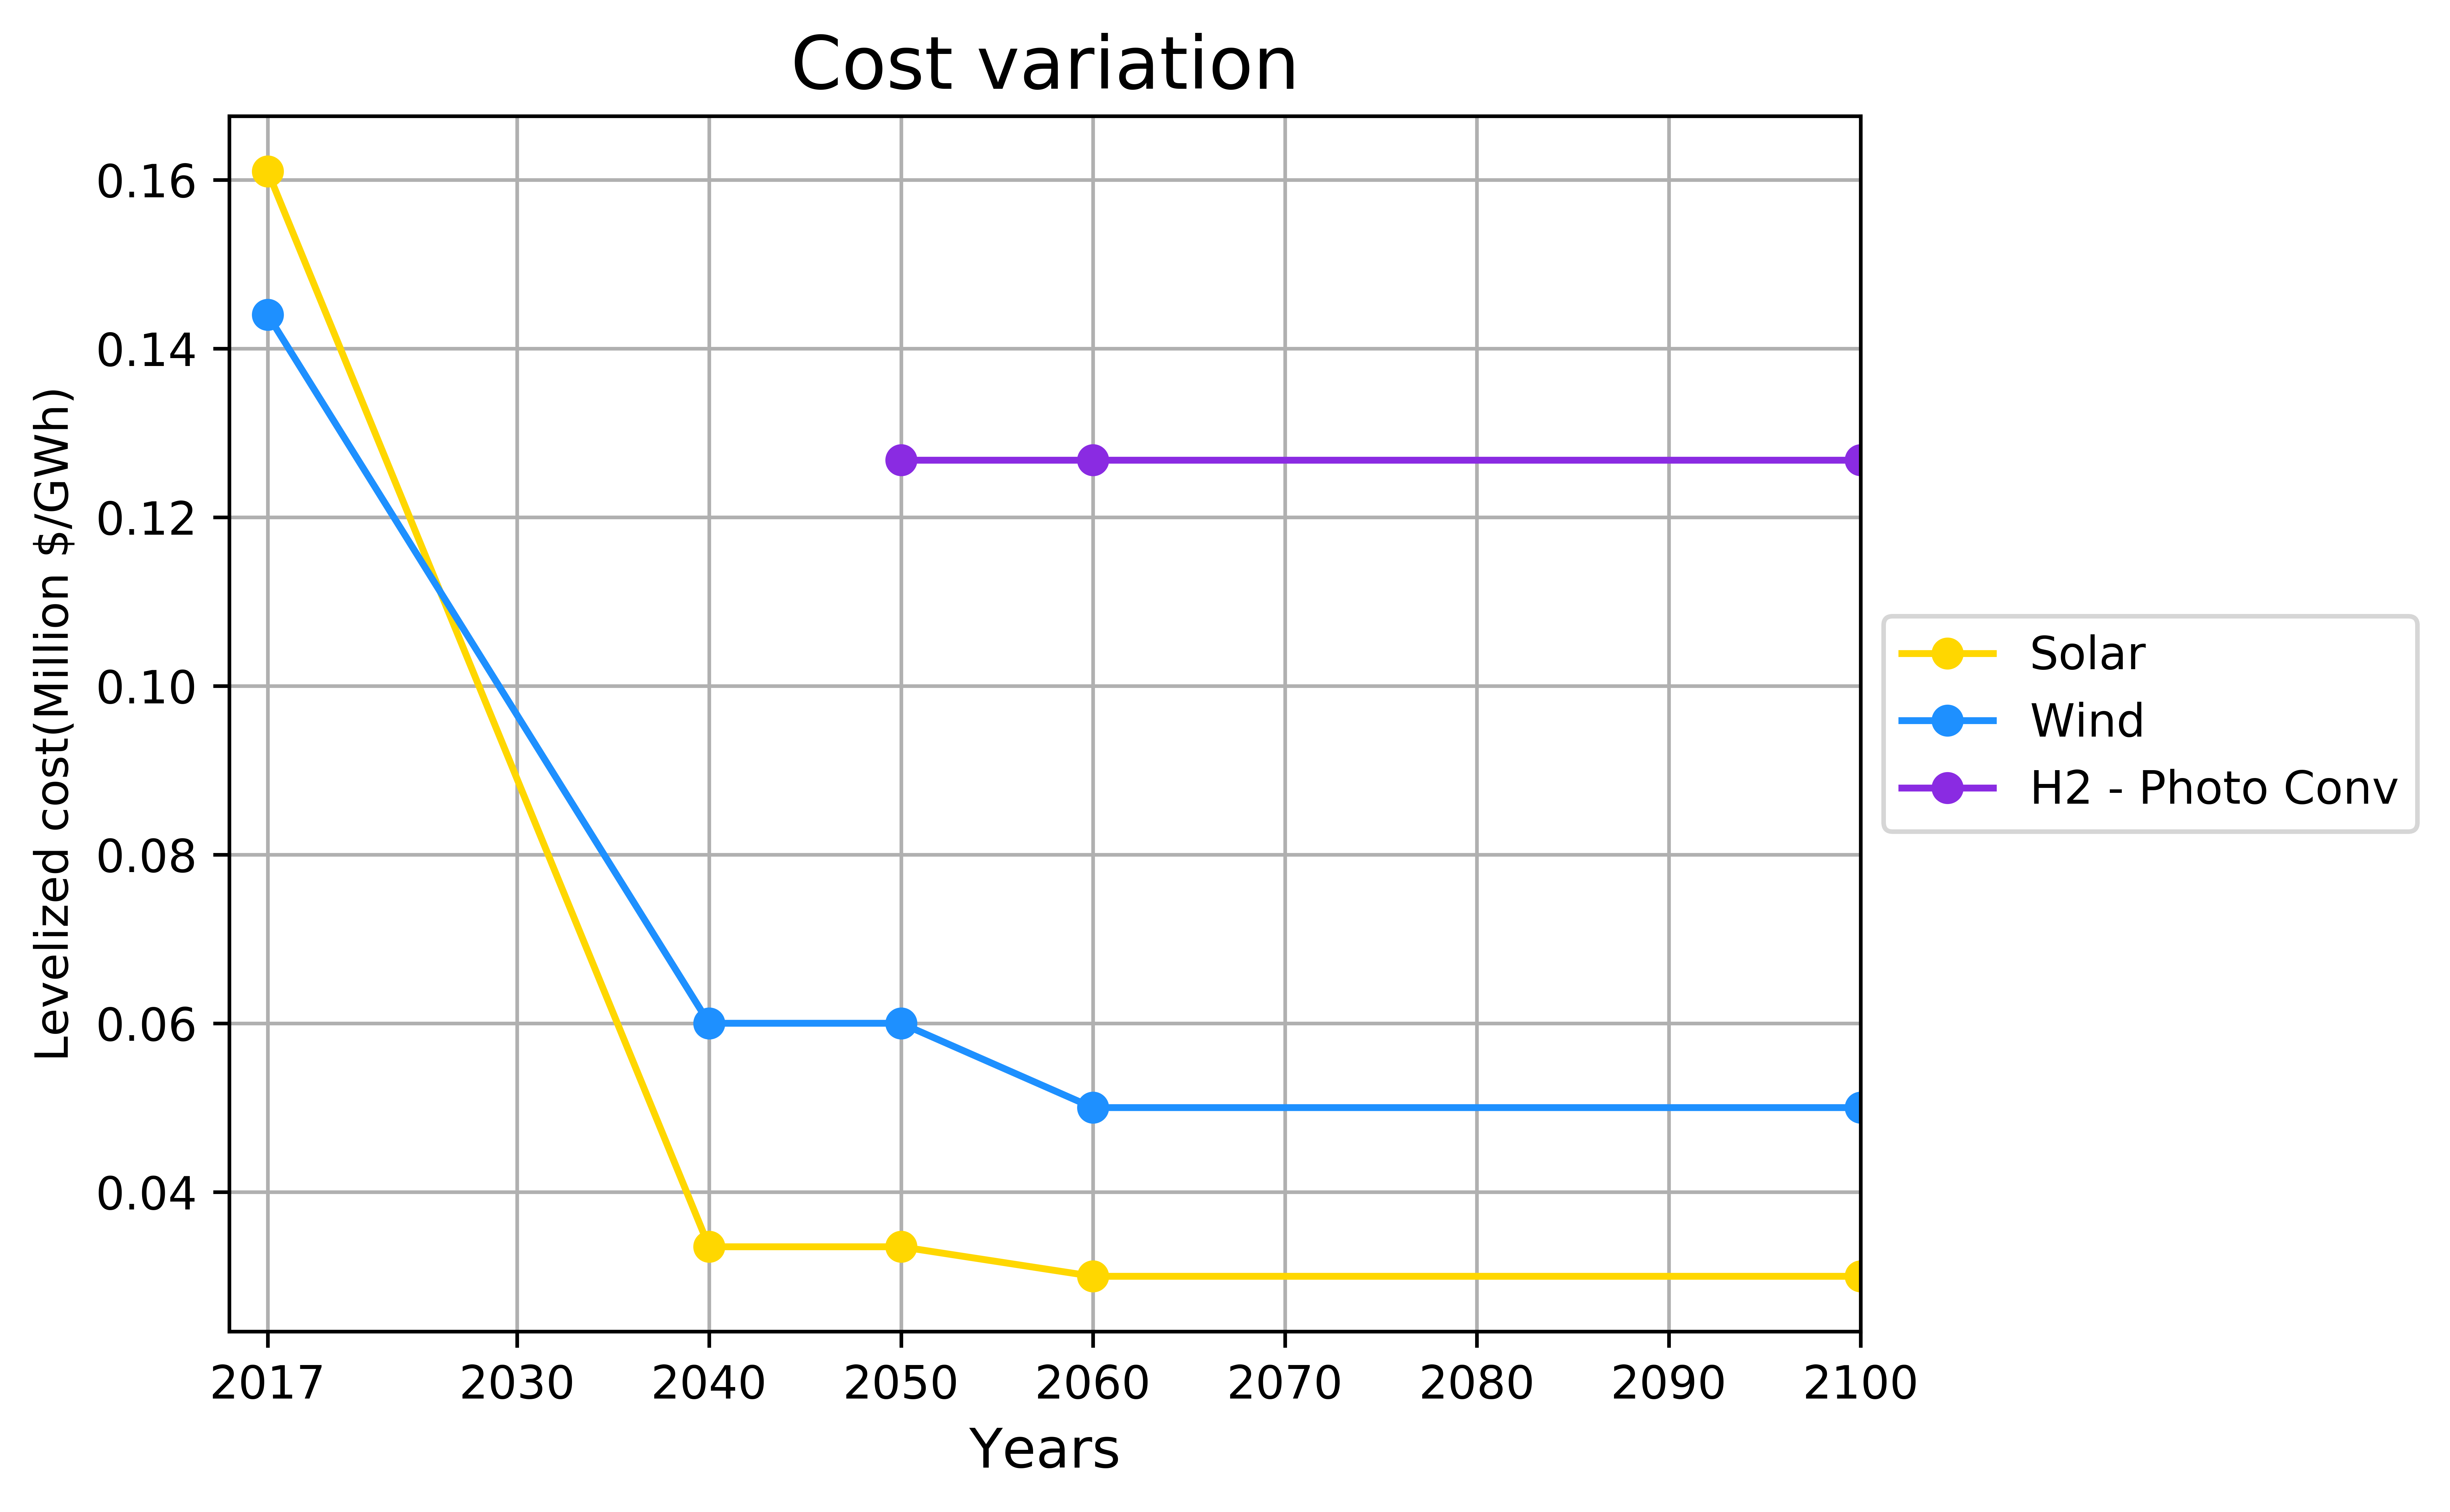
\includegraphics[scale=0.6]{./images/cost}
    \end{center}
          \caption{Cost variation of solar, wind, and H$_2$ production.}
    \label{cost}
  \end{figure}
\end{frame}
